The goal of \eTrice{} is to describe distributed systems on a logical level. In the current version not all 
elements will be used. But as prerequisite for further versions the following elements can be defined:
\begin{itemize}
\item the \textit{LogicalSystem} (currently optional)
\item at least one \textit{SubSystemClass} (mandatory)
\item at least one \textit{ActorClass} (mandatory)
\end{itemize}

The \textit{LogicalSystem} represents the complete distributed system and contains at least one 
\textit{SubSystemRef}. The \textit{SubSystemClass} represents an address space (e.g. a linux process or an image for a microcontroller) and contains at least one 
\textit{ActorRef}. The \textit{ActorClass} is the building block for building the hierachical structure of an application. 
A good point to start is to define a top level actor that can be used as structural root within the subsystem.

The outline view of the textual ROOM editor shows the main modeling elements in a navigation tree. You can jump to an element in the textual editor by double clicking the element in the outline view.

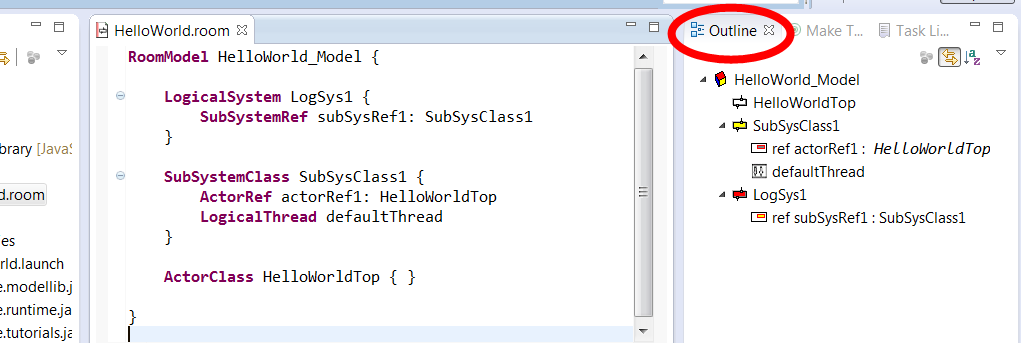
\includegraphics[width=0.8\textwidth]{images/015-HelloWorld02.png}
% !images/015-HelloWorld02.png!

\subsection{Create a state machine}

We will implement the Hello World code on the initial transition of the \textit{HelloWorldTop} actor. 
Therefore open the state machine editor by right clicking the \textit{HelloWorldTop} actor in the outline view and select \textit{Edit Behavior}.

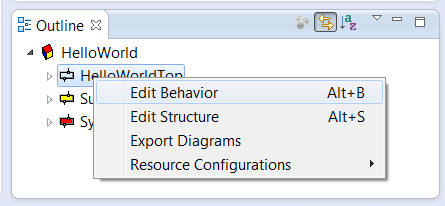
\includegraphics{images/015-HelloWorld03.png}
% !images/015-HelloWorld03.png!

The state machine editor will be opened. Drag and drop an \textit{Initial Point} from the tool box to the 
diagram into the top level state. Drag and drop a \textit{State} from the tool box to the diagram. Confirm the dialogue with \textit{ok}. Select the \textit{Transition} in the tool box and draw the transition from the \textit{Initial Point} to the State. Open the transition dialogue by double clicking the transition arrow and fill in the action code. Be aware of the different action code in Java and C.

\begin{figure}[ht]
\begin{minipage}[b]{0.45\linewidth}
	\begin{mdframed}
	\textbf{action code for Java}
	\begin{verbatim}
	System.out.println("Hello World !");
	\end{verbatim}
	\end{mdframed}
\end{minipage}
\hspace{0.5cm}
\begin{minipage}[b]{0.45\linewidth}
	\begin{mdframed}
	\textbf{action code for C}
	\begin{verbatim}
	printf("Hello World\n");
	\end{verbatim}
	\end{mdframed}
\end{minipage}
\end{figure}

 
The result should look like this:

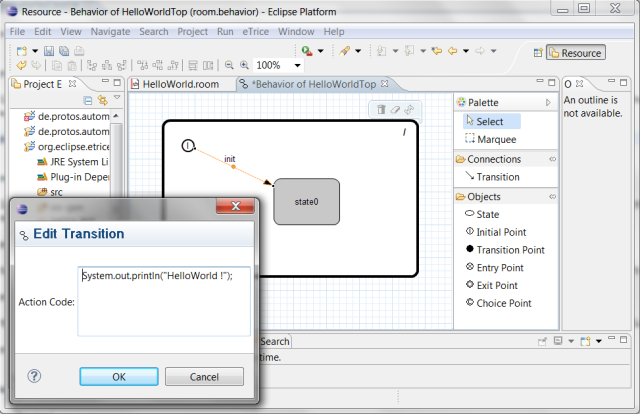
\includegraphics[width=0.8\textwidth]{images/015-HelloWorld04.png}
% !images/015-HelloWorld04.png!

Save the diagram and inspect the model (HelloWorld.room) file. Note that the textual representation was changed after saving 
the diagram.

\begin{figure}[ht]
\begin{minipage}[t]{0.50\linewidth}
\begin{mdframed}
	\textbf{room model for Java}
	\newline
\begin{lstlisting}[language=ROOM]
RoomModel HelloWorld_Model {
	LogicalSystem LogSys1 {
		SubSystemRef subSysRef1:SubSysClass1 
	}
	SubSystemClass SubSysClass1 {
		ActorRef actorRef1:HelloWorldTop 
		LogicalThread defaultThread
	}
	ActorClass HelloWorldTop {
		Structure { }
		Behavior {
			StateMachine {
				Transition init: initial -> state0 {
					action {
						"System.out.println(\"Hello World\");"
					}
				}
				State state0
			}
		}
	}
}
\end{lstlisting}
\end{mdframed}
\end{minipage}
\hspace{0.1cm}
\begin{minipage}[t]{0.50\linewidth}
\begin{mdframed}
	\textbf{room model for C}
	\newline
\begin{lstlisting}[language=ROOM]
RoomModel HelloWorld_Model {
	LogicalSystem LogSys1 {
		SubSystemRef subSysRef1: SubSysClass1
	}
	SubSystemClass SubSysClass1 {
		ActorRef actorRef1: HelloWorldTop
		LogicalThread defaultThread
	}
	ActorClass HelloWorldTop {
		Structure { }
		Behavior {
			StateMachine {
				Transition init: initial -> state0 {
					action {
						"printf(\"Hello World\\n\");"
					}
				}
				State state0
			}
		}
	}
}
\end{lstlisting}
\end{mdframed}
\end{minipage}
\end{figure}



